% Options for packages loaded elsewhere
\PassOptionsToPackage{unicode}{hyperref}
\PassOptionsToPackage{hyphens}{url}
%
\documentclass[
  12pt,
  a4paper,
]{article}
\usepackage{amsmath,amssymb}
\usepackage{setspace}
\usepackage{iftex}
\ifPDFTeX
  \usepackage[T1]{fontenc}
  \usepackage[utf8]{inputenc}
  \usepackage{textcomp} % provide euro and other symbols
\else % if luatex or xetex
  \usepackage{unicode-math} % this also loads fontspec
  \defaultfontfeatures{Scale=MatchLowercase}
  \defaultfontfeatures[\rmfamily]{Ligatures=TeX,Scale=1}
\fi
\usepackage{lmodern}
\ifPDFTeX\else
  % xetex/luatex font selection
\fi
% Use upquote if available, for straight quotes in verbatim environments
\IfFileExists{upquote.sty}{\usepackage{upquote}}{}
\IfFileExists{microtype.sty}{% use microtype if available
  \usepackage[]{microtype}
  \UseMicrotypeSet[protrusion]{basicmath} % disable protrusion for tt fonts
}{}
\makeatletter
\@ifundefined{KOMAClassName}{% if non-KOMA class
  \IfFileExists{parskip.sty}{%
    \usepackage{parskip}
  }{% else
    \setlength{\parindent}{0pt}
    \setlength{\parskip}{6pt plus 2pt minus 1pt}}
}{% if KOMA class
  \KOMAoptions{parskip=half}}
\makeatother
\usepackage{xcolor}
\usepackage[margin=1in]{geometry}
\usepackage{color}
\usepackage{fancyvrb}
\newcommand{\VerbBar}{|}
\newcommand{\VERB}{\Verb[commandchars=\\\{\}]}
\DefineVerbatimEnvironment{Highlighting}{Verbatim}{commandchars=\\\{\}}
% Add ',fontsize=\small' for more characters per line
\usepackage{framed}
\definecolor{shadecolor}{RGB}{248,248,248}
\newenvironment{Shaded}{\begin{snugshade}}{\end{snugshade}}
\newcommand{\AlertTok}[1]{\textcolor[rgb]{0.94,0.16,0.16}{#1}}
\newcommand{\AnnotationTok}[1]{\textcolor[rgb]{0.56,0.35,0.01}{\textbf{\textit{#1}}}}
\newcommand{\AttributeTok}[1]{\textcolor[rgb]{0.13,0.29,0.53}{#1}}
\newcommand{\BaseNTok}[1]{\textcolor[rgb]{0.00,0.00,0.81}{#1}}
\newcommand{\BuiltInTok}[1]{#1}
\newcommand{\CharTok}[1]{\textcolor[rgb]{0.31,0.60,0.02}{#1}}
\newcommand{\CommentTok}[1]{\textcolor[rgb]{0.56,0.35,0.01}{\textit{#1}}}
\newcommand{\CommentVarTok}[1]{\textcolor[rgb]{0.56,0.35,0.01}{\textbf{\textit{#1}}}}
\newcommand{\ConstantTok}[1]{\textcolor[rgb]{0.56,0.35,0.01}{#1}}
\newcommand{\ControlFlowTok}[1]{\textcolor[rgb]{0.13,0.29,0.53}{\textbf{#1}}}
\newcommand{\DataTypeTok}[1]{\textcolor[rgb]{0.13,0.29,0.53}{#1}}
\newcommand{\DecValTok}[1]{\textcolor[rgb]{0.00,0.00,0.81}{#1}}
\newcommand{\DocumentationTok}[1]{\textcolor[rgb]{0.56,0.35,0.01}{\textbf{\textit{#1}}}}
\newcommand{\ErrorTok}[1]{\textcolor[rgb]{0.64,0.00,0.00}{\textbf{#1}}}
\newcommand{\ExtensionTok}[1]{#1}
\newcommand{\FloatTok}[1]{\textcolor[rgb]{0.00,0.00,0.81}{#1}}
\newcommand{\FunctionTok}[1]{\textcolor[rgb]{0.13,0.29,0.53}{\textbf{#1}}}
\newcommand{\ImportTok}[1]{#1}
\newcommand{\InformationTok}[1]{\textcolor[rgb]{0.56,0.35,0.01}{\textbf{\textit{#1}}}}
\newcommand{\KeywordTok}[1]{\textcolor[rgb]{0.13,0.29,0.53}{\textbf{#1}}}
\newcommand{\NormalTok}[1]{#1}
\newcommand{\OperatorTok}[1]{\textcolor[rgb]{0.81,0.36,0.00}{\textbf{#1}}}
\newcommand{\OtherTok}[1]{\textcolor[rgb]{0.56,0.35,0.01}{#1}}
\newcommand{\PreprocessorTok}[1]{\textcolor[rgb]{0.56,0.35,0.01}{\textit{#1}}}
\newcommand{\RegionMarkerTok}[1]{#1}
\newcommand{\SpecialCharTok}[1]{\textcolor[rgb]{0.81,0.36,0.00}{\textbf{#1}}}
\newcommand{\SpecialStringTok}[1]{\textcolor[rgb]{0.31,0.60,0.02}{#1}}
\newcommand{\StringTok}[1]{\textcolor[rgb]{0.31,0.60,0.02}{#1}}
\newcommand{\VariableTok}[1]{\textcolor[rgb]{0.00,0.00,0.00}{#1}}
\newcommand{\VerbatimStringTok}[1]{\textcolor[rgb]{0.31,0.60,0.02}{#1}}
\newcommand{\WarningTok}[1]{\textcolor[rgb]{0.56,0.35,0.01}{\textbf{\textit{#1}}}}
\usepackage{longtable,booktabs,array}
\usepackage{calc} % for calculating minipage widths
% Correct order of tables after \paragraph or \subparagraph
\usepackage{etoolbox}
\makeatletter
\patchcmd\longtable{\par}{\if@noskipsec\mbox{}\fi\par}{}{}
\makeatother
% Allow footnotes in longtable head/foot
\IfFileExists{footnotehyper.sty}{\usepackage{footnotehyper}}{\usepackage{footnote}}
\makesavenoteenv{longtable}
\usepackage{graphicx}
\makeatletter
\def\maxwidth{\ifdim\Gin@nat@width>\linewidth\linewidth\else\Gin@nat@width\fi}
\def\maxheight{\ifdim\Gin@nat@height>\textheight\textheight\else\Gin@nat@height\fi}
\makeatother
% Scale images if necessary, so that they will not overflow the page
% margins by default, and it is still possible to overwrite the defaults
% using explicit options in \includegraphics[width, height, ...]{}
\setkeys{Gin}{width=\maxwidth,height=\maxheight,keepaspectratio}
% Set default figure placement to htbp
\makeatletter
\def\fps@figure{htbp}
\makeatother
\setlength{\emergencystretch}{3em} % prevent overfull lines
\providecommand{\tightlist}{%
  \setlength{\itemsep}{0pt}\setlength{\parskip}{0pt}}
\setcounter{secnumdepth}{5}
\newlength{\cslhangindent}
\setlength{\cslhangindent}{1.5em}
\newlength{\csllabelwidth}
\setlength{\csllabelwidth}{3em}
\newlength{\cslentryspacingunit} % times entry-spacing
\setlength{\cslentryspacingunit}{\parskip}
\newenvironment{CSLReferences}[2] % #1 hanging-ident, #2 entry spacing
 {% don't indent paragraphs
  \setlength{\parindent}{0pt}
  % turn on hanging indent if param 1 is 1
  \ifodd #1
  \let\oldpar\par
  \def\par{\hangindent=\cslhangindent\oldpar}
  \fi
  % set entry spacing
  \setlength{\parskip}{#2\cslentryspacingunit}
 }%
 {}
\usepackage{calc}
\newcommand{\CSLBlock}[1]{#1\hfill\break}
\newcommand{\CSLLeftMargin}[1]{\parbox[t]{\csllabelwidth}{#1}}
\newcommand{\CSLRightInline}[1]{\parbox[t]{\linewidth - \csllabelwidth}{#1}\break}
\newcommand{\CSLIndent}[1]{\hspace{\cslhangindent}#1}
\newcommand{\docTitle}{PB Tables}
\usepackage{pgfplots}
\usepackage{fvextra}
\DefineVerbatimEnvironment{Highlighting}{Verbatim}{breaklines,commandchars=\\\{\}}
\usepackage[skins]{tcolorbox}
\usepackage{listings}
\usepackage{booktabs}
\usepackage{listings}
\usepackage{setspace}
\usepackage{titling}
\pgfplotsset{compat=1.18}
\usepackage{tikz}
\usepackage{tikz-3dplot}
\usetikzlibrary{arrows}
\usepackage{xcolor}
\usepackage{etoolbox}
\usepackage{amsmath}
\usepackage{caption}
\usepackage{enumitem}
\usepackage{varwidth}
\usepackage{mathrsfs}
\usepackage[nochapter, tocentry, owncaptions, tablegrid]{vhistory}
\usepackage{tasks}
\usepackage{scrlayer-scrpage}
\numberwithin{equation}{section}
\usepackage{lastpage}
\captionsetup[figure]{font=small,labelfont=small}
\usepackage{amsthm}
\theoremstyle{plain}
\newtheorem{theorem}{Theorem}
\theoremstyle{definition}
\newtheorem{defn}{Definition}
\newtheorem{xmpl}{Example}
\theoremstyle{remark}
\newtheorem{remark}{Remark}
\newtheorem{algorithm}{Algorithm} 
\newtheoremstyle{note}    % style name
{2ex}                     % above space
{2ex}                     % below space
{}                        % body font
{}                        % indent amount
{\scshape}                % head font
{.}                       % post head punctuation
{\newline}                % post head punctuation
{}                        % head spec
\theoremstyle{note}
\newtheorem{scnote}{Note}  

\pretitle{%
\begin{flushleft} \LARGE
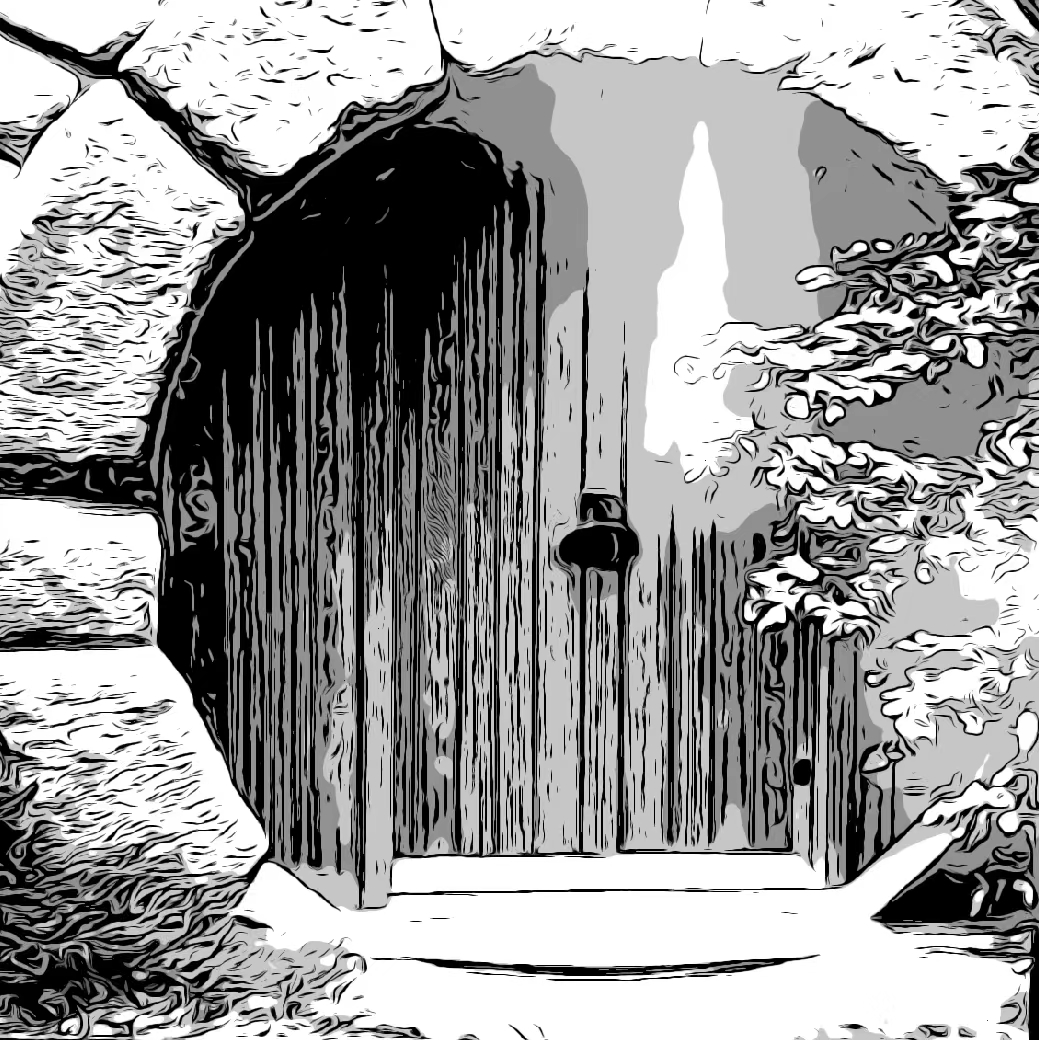
\includegraphics[width=2cm,height=2cm]{IH2.jpg}
\end{flushleft}
\begin{flushright} \LARGE
}

\posttitle{\end{flushright}}
\preauthor{\begin{flushright}}
\postauthor{\end{flushright}}
\predate{\begin{flushright}}
\postdate{\end{flushright}}

\ohead[]{IH - AppliedMath WhitePaper}
\ifoot{\hsize=350pt \docTitle\ -- Version \vhCurrentVersion}
\ofoot{\thepage~/~\pageref{LastPage}}
\cfoot[]{}

\ifLuaTeX
  \usepackage{selnolig}  % disable illegal ligatures
\fi
\IfFileExists{bookmark.sty}{\usepackage{bookmark}}{\usepackage{hyperref}}
\IfFileExists{xurl.sty}{\usepackage{xurl}}{} % add URL line breaks if available
\urlstyle{same}
\hypersetup{
  pdftitle={Plackett-Burman Tables},
  pdfauthor={Donald Palahnuk},
  hidelinks,
  pdfcreator={LaTeX via pandoc}}

\title{Plackett-Burman Tables}
\usepackage{etoolbox}
\makeatletter
\providecommand{\subtitle}[1]{% add subtitle to \maketitle
  \apptocmd{\@title}{\par {\large #1 \par}}{}{}
}
\makeatother
\subtitle{\textit{fF2 vs PB Tables, low $n$}}
\author{Donald Palahnuk}
\date{\vhCurrentDate\\
version \vhCurrentVersion\\
\strut \\
InsightHatch WhitePaper: fF2 vs PB Tables For (low \(n\))\\
\textbf{IH-fF2 PB Tables-v}\textbf{\vhCurrentVersion}}

\begin{document}
\maketitle

{
\setcounter{tocdepth}{2}
\tableofcontents
}
\setstretch{1.25}
\hfill\break

\begin{versionhistory}
  \vhEntry{0.0}{2023.10.10}{DP}{created!}
  \vhEntry{0.1}{2023.10.10}{DP}{compared fF2 vs PB calls, added kable tables}
  \vhEntry{0.2}{2023.10.11}{DP}{add resolution, and some math}
  \vhEntry{1.0}{2024.10.27}{DP}{update for github issue}
\end{versionhistory}

\newpage

\hypertarget{fractional-factorial-and-plackett-burman-doe}{%
\section{Fractional Factorial and Plackett-Burman
DOE}\label{fractional-factorial-and-plackett-burman-doe}}

Design of Experiments (DOE) is a methodological framework for
systemically planning experiments, collecting data, and analyzing
results. 2 Level Fractional Factorial (fF2) and Plackett-Burman (PB)
designs are two common techniques within DOE that aim to reduce the
number of experiments you need to run when investigating multiple
factors.

\hypertarget{difference-between-fractional-factorial-and-plackett-burman-design}{%
\subsection{Difference between Fractional Factorial and Plackett-Burman
Design}\label{difference-between-fractional-factorial-and-plackett-burman-design}}

\hypertarget{fractional-factorial-ff2-2-level-design}{%
\subsubsection{Fractional Factorial (fF2) 2 Level
Design}\label{fractional-factorial-ff2-2-level-design}}

In a full factorial (FF) design, you study all possible combinations of
the factors. However, this can become impractical with a large number of
factors. In a fractional factorial design, only a ``fraction'' of the
full set of experiments is carried out. The fraction is chosen carefully
so that certain effects (main effects or interactions) can still be
estimated. Note in this write-up we use the conventions:
\(n = 2^{(f-r)}\), where \(f\)=factors, \(r\)=reductions).

Variable Resolution: Fractional factorial designs can be of various
resolutions (III, IV, V, etc.), depending on how you fractionate the
full factorial design.

Resolution III: Main effects are confounded with two-factor interactions
but not with each other.

Resolution IV: Main effects are clear of all two-factor interactions.
Two-factor interactions are confounded with each other but not with main
effects.

Resolution V and above: Higher resolutions allow you to separate
higher-order interactions from lower-order effects.

\hypertarget{plackett-burman-design}{%
\subsubsection{Plackett-Burman Design}\label{plackett-burman-design}}

The Plackett-Burman design is another approach to reducing the number of
experimental runs. It's commonly used for screening experiments where
you have many factors and you want to identify which ones have
significant effects on the outcome. These designs are specialized for
estimating main effects and \textbf{assume that interaction effects are
negligible.}

Resolution III: Plackett-Burman designs are generally resolution III
designs. This means that main effects are confounded with two-factor
interactions but not with each other. In other words, you cannot
distinguish between a main effect and a two-factor interaction that it
is confounded with. However, main effects are clear of each other.

\hypertarget{pros-and-cons}{%
\subsection{\texorpdfstring{\emph{Pros} and
\emph{Cons}}{Pros and Cons}}\label{pros-and-cons}}

\hypertarget{fractional-factorial-design}{%
\subsubsection{Fractional Factorial
Design}\label{fractional-factorial-design}}

\emph{Pros:} More flexible in terms of defining the ``fraction'' of
experiments. Allows for the estimation of interaction effects. Can be
optimal or near-optimal for a given effect size and error.

\emph{Cons:} More complex to set up and analyze, especially for
higher-order fractions. Not efficient for screening a large number of
factors, especially when most are not influential.

\hypertarget{plackett-burman-design-1}{%
\subsubsection{Plackett-Burman Design}\label{plackett-burman-design-1}}

\emph{Pros:} Simple to set up and analyze. Efficient for screening a
large number of factors to identify the few that are most significant.

\emph{Cons:} Assumes that interaction effects are negligible, which may
not be true. Less flexible in design choices compared to fractional
factorial.

In summary, fractional factorial designs offer more flexibility and the
ability to study interactions but can be complex and often require more
runs than Plackett-Burman designs. Plackett-Burman designs are more
straightforward and are generally used for initial screening when you
have a large number of factors and you want to identify the most
significant ones quickly.

\hypertarget{discussion-of-increasing-n-in-the-context-of-ff2-pb-designs.}{%
\subsection{\texorpdfstring{Discussion of increasing \(n\) in the
context of fF2 \& PB
designs.}{Discussion of increasing n in the context of fF2 \& PB designs.}}\label{discussion-of-increasing-n-in-the-context-of-ff2-pb-designs.}}

The quality of multivariate residuals \((y\hat - y)\) in a Design of
Experiments (DOE) largely depends on the underlying structure of the
problem, the number and nature of factors, and the presence of
interactions and higher-order effects. Here's a breakdown based on the
two designs you've mentioned:

Lets discuss a fF2 of \(n=12\) vs PB of \(n=8\) runs to further
understand how these concepts manifest.

\emph{fF2 with 12 Runs:} A 12-run fF2 design will generally allow you to
estimate more effects (both main effects and interactions) than an 8-run
PB design. This would generally make the model fit better to the actual
observed data, potentially yielding better residuals.

\emph{PB with 8 Runs:} An 8-run PB design is generally intended for
screening a large number of factors to find the few that are most
significant. It is usually not efficient for estimating interaction
effects, so if your process has significant interactions, a
Plackett-Burman design might not capture them well, leading to poorer
residuals. However, it allows for a reduced number of experiments which
can help to save in experimental execution costs.

\emph{Key Points to Consider:}

\emph{Interactions:} If interactions between factors are significant, a
fractional factorial design would generally yield better residuals as it
allows for the estimation of interactions.

\emph{Number of Factors:} The Plackett-Burman design is useful for
screening a large number of factors. If most factors are not
influential, then a Plackett-Burman design may perform reasonably well
even with fewer runs.

\emph{Assumptions:} Plackett-Burman assumes negligible interactions. If
this assumption holds true, then it may give good residuals even with
fewer runs.

\emph{Model Complexity:} Fractional Factorial designs are generally more
flexible and can fit more complex models than Plackett-Burman designs.

In summary, if you believe your system is better represented by a model
that includes interaction terms, or if you want to estimate these terms,
a 12-run fractional factorial design is more likely to give better
multivariate residuals. On the other hand, if you are primarily
interested in identifying the main effects quickly and cheaply, and are
willing to assume that interactions are negligible, then an 8-run
Plackett-Burman design could suffice.

\newpage

\hypertarget{ff2-vs-pb-in-terms-of-base-design-n-experiments-and-f-factors}{%
\section{\texorpdfstring{fF2 vs PB in terms of base design \(n\)
experiments and \(f\)
factors}{fF2 vs PB in terms of base design n experiments and f factors}}\label{ff2-vs-pb-in-terms-of-base-design-n-experiments-and-f-factors}}

Comparison of \(n\) between Plackett-Burman and
\(2_{\mathrm{III}}^{f-r}\)

\begin{center}
\begin{tabular}{|c|c|c|}
\hline Number of factors & PB & fF2 III \\
\hline $4 \leq f \leq 7$ & 8 & 8 \\
\hline $8 \leq f \leq 11$ & 12 & 16 \\
\hline $12 \leq f \leq 15$ & 16 & 16 \\
\hline $16 \leq f \leq 19$ & 20 & 32 \\
\hline $20 \leq f \leq 23$ & 24 & 32 \\
\hline $24 \leq f \leq 27$ & 28 & 32 \\
\hline $28 \leq f \leq 31$ & 32 & 32 \\
\hline $32 \leq f \leq 35$ & 36 & 64 \\
\hline$\vdots$ & $\vdots$ & $\vdots$ \\
\hline $64 \leq f \leq 67$ & 68 & 128 \\
\hline
\end{tabular}
\end{center}

\hypertarget{ff2-pb-tables-set-for-4-and-5-factors}{%
\section{fF2 \& PB Tables Set for 4 and 5
factors}\label{ff2-pb-tables-set-for-4-and-5-factors}}

Series of low \(n\) Placket-Burman and fF2 (reduced factorial) Design
Tables

\begin{itemize}
\tightlist
\item
  Motivation: Develop reference of commonly used fF2 \& PB Tables for
  typical BioProcess PD work
\item
  Compile Interesting Examples - for useful consideration
\end{itemize}

\hypertarget{comments}{%
\subsection{Comments}\label{comments}}

\hypertarget{pb-designs}{%
\subsubsection{PB Designs}\label{pb-designs}}

PB designs are done in increments of 4 \ldots{} \(n\) = 4, 8, 12, etc.

\hypertarget{ff2-designs}{%
\subsubsection{fF2 Designs}\label{ff2-designs}}

fF2 designs are based on powers of 2 (\(2^{(f-r)}\), where
\(f\)=factors, \(r\)=reductions) \ldots{} \(n\) = 4, 8, 16, etc. (or if
not a power of 2 -\textgreater{} design must be truncated)

\newpage

\hypertarget{ff2-pb-for-4-factors}{%
\section{fF2 \& PB for 4 Factors}\label{ff2-pb-for-4-factors}}

\setcounter{table}{0}

\hypertarget{pb-vs-ff2-8-runs-4-factors}{%
\subsection{PB vs fF2 8 runs, 4
factors}\label{pb-vs-ff2-8-runs-4-factors}}

\begin{Shaded}
\begin{Highlighting}[]
\FunctionTok{library}\NormalTok{(}\StringTok{"FrF2"}\NormalTok{)}
\NormalTok{design }\OtherTok{\textless{}{-}} \FunctionTok{pb}\NormalTok{(}\DecValTok{8}\NormalTok{, }\DecValTok{4}\NormalTok{)}
\NormalTok{knitr}\SpecialCharTok{::}\FunctionTok{kable}\NormalTok{(design, }\AttributeTok{align =} \StringTok{"rrrr"}\NormalTok{, }\AttributeTok{caption =} \StringTok{"PB, n=8, f=4"}\NormalTok{)}
\end{Highlighting}
\end{Shaded}

\begin{longtable}[]{@{}rrrr@{}}
\caption{PB, n=8, f=4}\tabularnewline
\toprule\noalign{}
A & B & C & D \\
\midrule\noalign{}
\endfirsthead
\toprule\noalign{}
A & B & C & D \\
\midrule\noalign{}
\endhead
\bottomrule\noalign{}
\endlastfoot
-1 & -1 & 1 & 1 \\
1 & 1 & -1 & -1 \\
-1 & -1 & -1 & -1 \\
-1 & 1 & 1 & -1 \\
1 & 1 & 1 & 1 \\
1 & -1 & -1 & 1 \\
-1 & 1 & -1 & 1 \\
1 & -1 & 1 & -1 \\
\end{longtable}

\begin{Shaded}
\begin{Highlighting}[]
\FunctionTok{library}\NormalTok{(}\StringTok{"FrF2"}\NormalTok{)}
\NormalTok{design }\OtherTok{\textless{}{-}} \FunctionTok{FrF2}\NormalTok{(}\DecValTok{8}\NormalTok{, }\DecValTok{4}\NormalTok{)}
\NormalTok{knitr}\SpecialCharTok{::}\FunctionTok{kable}\NormalTok{(design, }\AttributeTok{align =} \StringTok{"rrrr"}\NormalTok{, }\AttributeTok{caption =} \StringTok{"fF, n=8, f=4"}\NormalTok{)}
\end{Highlighting}
\end{Shaded}

\begin{longtable}[]{@{}rrrr@{}}
\caption{fF, n=8, f=4}\tabularnewline
\toprule\noalign{}
A & B & C & D \\
\midrule\noalign{}
\endfirsthead
\toprule\noalign{}
A & B & C & D \\
\midrule\noalign{}
\endhead
\bottomrule\noalign{}
\endlastfoot
-1 & 1 & -1 & 1 \\
1 & -1 & -1 & 1 \\
-1 & 1 & 1 & -1 \\
1 & -1 & 1 & -1 \\
1 & 1 & 1 & 1 \\
-1 & -1 & -1 & -1 \\
1 & 1 & -1 & -1 \\
-1 & -1 & 1 & 1 \\
\end{longtable}

\newpage

\hypertarget{pb-vs-ff2-1216-runs-4-factors}{%
\subsection{PB vs fF2 12/16 runs, 4
factors}\label{pb-vs-ff2-1216-runs-4-factors}}

\begin{Shaded}
\begin{Highlighting}[]
\FunctionTok{library}\NormalTok{(}\StringTok{"FrF2"}\NormalTok{)}
\NormalTok{design }\OtherTok{\textless{}{-}} \FunctionTok{pb}\NormalTok{(}\DecValTok{12}\NormalTok{, }\DecValTok{4}\NormalTok{)}
\NormalTok{knitr}\SpecialCharTok{::}\FunctionTok{kable}\NormalTok{(design, }\AttributeTok{align =} \StringTok{"rrrr"}\NormalTok{, }\AttributeTok{caption =} \StringTok{"PB, n=12, f=4"}\NormalTok{)}
\end{Highlighting}
\end{Shaded}

\begin{longtable}[]{@{}rrrr@{}}
\caption{PB, n=12, f=4}\tabularnewline
\toprule\noalign{}
A & B & C & D \\
\midrule\noalign{}
\endfirsthead
\toprule\noalign{}
A & B & C & D \\
\midrule\noalign{}
\endhead
\bottomrule\noalign{}
\endlastfoot
1 & 1 & -1 & -1 \\
-1 & 1 & 1 & 1 \\
1 & -1 & -1 & -1 \\
1 & 1 & 1 & -1 \\
1 & 1 & -1 & 1 \\
-1 & -1 & -1 & 1 \\
1 & -1 & 1 & 1 \\
1 & -1 & 1 & 1 \\
-1 & -1 & -1 & -1 \\
-1 & -1 & 1 & -1 \\
-1 & 1 & -1 & 1 \\
-1 & 1 & 1 & -1 \\
\end{longtable}

\begin{Shaded}
\begin{Highlighting}[]
\FunctionTok{library}\NormalTok{(}\StringTok{"FrF2"}\NormalTok{)}
\NormalTok{design }\OtherTok{\textless{}{-}} \FunctionTok{FrF2}\NormalTok{(}\DecValTok{16}\NormalTok{, }\DecValTok{4}\NormalTok{)}
\NormalTok{knitr}\SpecialCharTok{::}\FunctionTok{kable}\NormalTok{(design, }\AttributeTok{align =} \StringTok{"rrrr"}\NormalTok{, }\AttributeTok{caption =} \StringTok{"fF, n=12, f=4"}\NormalTok{)}
\end{Highlighting}
\end{Shaded}

\begin{longtable}[]{@{}rrrr@{}}
\caption{fF, n=12, f=4}\tabularnewline
\toprule\noalign{}
A & B & C & D \\
\midrule\noalign{}
\endfirsthead
\toprule\noalign{}
A & B & C & D \\
\midrule\noalign{}
\endhead
\bottomrule\noalign{}
\endlastfoot
-1 & -1 & 1 & 1 \\
1 & 1 & 1 & -1 \\
1 & 1 & -1 & -1 \\
-1 & -1 & -1 & -1 \\
1 & -1 & -1 & 1 \\
-1 & 1 & 1 & 1 \\
1 & -1 & -1 & -1 \\
1 & 1 & 1 & 1 \\
-1 & -1 & 1 & -1 \\
-1 & 1 & -1 & 1 \\
1 & 1 & -1 & 1 \\
-1 & 1 & -1 & -1 \\
1 & -1 & 1 & 1 \\
-1 & -1 & -1 & 1 \\
-1 & 1 & 1 & -1 \\
1 & -1 & 1 & -1 \\
\end{longtable}

\newpage

\hypertarget{ff2-pb-for-5-factors}{%
\section{fF2 \& PB for 5 Factors}\label{ff2-pb-for-5-factors}}

\hypertarget{pb-vs-ff2-8-runs-5-factors}{%
\subsection{PB vs fF2 8 runs, 5
factors}\label{pb-vs-ff2-8-runs-5-factors}}

\begin{Shaded}
\begin{Highlighting}[]
\FunctionTok{library}\NormalTok{(}\StringTok{"FrF2"}\NormalTok{)}
\NormalTok{design }\OtherTok{\textless{}{-}} \FunctionTok{pb}\NormalTok{(}\DecValTok{8}\NormalTok{, }\DecValTok{5}\NormalTok{)}
\NormalTok{knitr}\SpecialCharTok{::}\FunctionTok{kable}\NormalTok{(design, }\AttributeTok{align =} \StringTok{"rrrrr"}\NormalTok{, }\AttributeTok{caption =} \StringTok{"PB, n=8, f=5"}\NormalTok{)}
\end{Highlighting}
\end{Shaded}

\begin{longtable}[]{@{}rrrrr@{}}
\caption{PB, n=8, f=5}\tabularnewline
\toprule\noalign{}
A & B & C & D & E \\
\midrule\noalign{}
\endfirsthead
\toprule\noalign{}
A & B & C & D & E \\
\midrule\noalign{}
\endhead
\bottomrule\noalign{}
\endlastfoot
1 & -1 & 1 & -1 & -1 \\
-1 & -1 & -1 & -1 & -1 \\
-1 & 1 & -1 & -1 & 1 \\
1 & 1 & -1 & 1 & -1 \\
1 & 1 & 1 & -1 & 1 \\
-1 & 1 & 1 & 1 & -1 \\
1 & -1 & -1 & 1 & 1 \\
-1 & -1 & 1 & 1 & 1 \\
\end{longtable}

\begin{Shaded}
\begin{Highlighting}[]
\FunctionTok{library}\NormalTok{(}\StringTok{"FrF2"}\NormalTok{)}
\NormalTok{design }\OtherTok{\textless{}{-}} \FunctionTok{FrF2}\NormalTok{(}\DecValTok{8}\NormalTok{, }\DecValTok{5}\NormalTok{)}
\NormalTok{knitr}\SpecialCharTok{::}\FunctionTok{kable}\NormalTok{(design, }\AttributeTok{align =} \StringTok{"rrrrr"}\NormalTok{, }\AttributeTok{caption =} \StringTok{"fF, n=8, f=5"}\NormalTok{)}
\end{Highlighting}
\end{Shaded}

\begin{longtable}[]{@{}rrrrr@{}}
\caption{fF, n=8, f=5}\tabularnewline
\toprule\noalign{}
A & B & C & D & E \\
\midrule\noalign{}
\endfirsthead
\toprule\noalign{}
A & B & C & D & E \\
\midrule\noalign{}
\endhead
\bottomrule\noalign{}
\endlastfoot
1 & 1 & -1 & 1 & -1 \\
-1 & -1 & -1 & 1 & 1 \\
1 & -1 & 1 & -1 & 1 \\
-1 & -1 & 1 & 1 & -1 \\
-1 & 1 & 1 & -1 & -1 \\
1 & 1 & 1 & 1 & 1 \\
1 & -1 & -1 & -1 & -1 \\
-1 & 1 & -1 & -1 & 1 \\
\end{longtable}

\newpage

\hypertarget{pb-vs-ff2-12-runs-5-factors}{%
\subsection{PB vs fF2 12 runs, 5
factors}\label{pb-vs-ff2-12-runs-5-factors}}

\begin{Shaded}
\begin{Highlighting}[]
\FunctionTok{library}\NormalTok{(}\StringTok{"FrF2"}\NormalTok{)}
\NormalTok{design }\OtherTok{\textless{}{-}} \FunctionTok{pb}\NormalTok{(}\DecValTok{12}\NormalTok{, }\DecValTok{5}\NormalTok{)}
\NormalTok{knitr}\SpecialCharTok{::}\FunctionTok{kable}\NormalTok{(design, }\AttributeTok{align =} \StringTok{"rrrr"}\NormalTok{, }\AttributeTok{caption =} \StringTok{"PB, n=12, f=5"}\NormalTok{)}
\end{Highlighting}
\end{Shaded}

\begin{longtable}[]{@{}rrrrr@{}}
\caption{PB, n=12, f=5}\tabularnewline
\toprule\noalign{}
A & B & C & D & E \\
\midrule\noalign{}
\endfirsthead
\toprule\noalign{}
A & B & C & D & E \\
\midrule\noalign{}
\endhead
\bottomrule\noalign{}
\endlastfoot
1 & -1 & 1 & 1 & -1 \\
-1 & 1 & -1 & 1 & 1 \\
1 & -1 & 1 & 1 & 1 \\
-1 & -1 & 1 & -1 & 1 \\
1 & 1 & 1 & -1 & -1 \\
1 & 1 & -1 & 1 & 1 \\
1 & -1 & -1 & -1 & 1 \\
-1 & 1 & 1 & 1 & -1 \\
-1 & -1 & -1 & 1 & -1 \\
-1 & 1 & 1 & -1 & 1 \\
-1 & -1 & -1 & -1 & -1 \\
1 & 1 & -1 & -1 & -1 \\
\end{longtable}

\begin{Shaded}
\begin{Highlighting}[]
\FunctionTok{library}\NormalTok{(}\StringTok{"FrF2"}\NormalTok{)}
\NormalTok{design }\OtherTok{\textless{}{-}} \FunctionTok{FrF2}\NormalTok{(}\DecValTok{16}\NormalTok{, }\DecValTok{5}\NormalTok{)}
\NormalTok{knitr}\SpecialCharTok{::}\FunctionTok{kable}\NormalTok{(design, }\AttributeTok{align =} \StringTok{"rrrr"}\NormalTok{, }\AttributeTok{caption =} \StringTok{"fF, n=12, f=5"}\NormalTok{)}
\end{Highlighting}
\end{Shaded}

\begin{longtable}[]{@{}rrrrr@{}}
\caption{fF, n=12, f=5}\tabularnewline
\toprule\noalign{}
A & B & C & D & E \\
\midrule\noalign{}
\endfirsthead
\toprule\noalign{}
A & B & C & D & E \\
\midrule\noalign{}
\endhead
\bottomrule\noalign{}
\endlastfoot
1 & -1 & 1 & 1 & -1 \\
1 & -1 & 1 & -1 & 1 \\
1 & -1 & -1 & -1 & -1 \\
-1 & -1 & 1 & -1 & -1 \\
-1 & 1 & -1 & -1 & -1 \\
1 & -1 & -1 & 1 & 1 \\
-1 & -1 & 1 & 1 & 1 \\
-1 & -1 & -1 & 1 & -1 \\
-1 & 1 & 1 & 1 & -1 \\
1 & 1 & -1 & 1 & -1 \\
-1 & -1 & -1 & -1 & 1 \\
1 & 1 & 1 & 1 & 1 \\
-1 & 1 & -1 & 1 & 1 \\
-1 & 1 & 1 & -1 & 1 \\
1 & 1 & -1 & -1 & 1 \\
1 & 1 & 1 & -1 & -1 \\
\end{longtable}

\newpage

\hypertarget{hadamard-matrix}{%
\section{Hadamard Matrix}\label{hadamard-matrix}}

In mathematics, a Hadamard matrix, named after the French mathematician
Jacques Hadamard, is a square matrix whose entries are either +1 or -1
and whose rows are mutually orthogonal. In geometric terms, this means
that each pair of rows in a Hadamard matrix represents two perpendicular
vectors, while in combinatorial terms, it means that each pair of rows
has matching entries in exactly half of their columns and mismatched
entries in the remaining columns. It is a consequence of this definition
that the corresponding properties hold for columns as well as rows.

The \(n\)-dimensional parallelotope spanned by the rows of an
\(n \times n\) Hadamard matrix has the
\underline{maximum possible $n$ dimensional volume among parallelotopes}
spanned by vectors whose entries are bounded in absolute value by 1.
Equivalently, a Hadamard matrix has maximal determinant among matrices
with entries of absolute value less than or equal to 1 and so is an
extremal solution of Hadamard's maximal determinant problem.

Let \(H\) be a Hadamard matrix of order \(n\). The transpose of \(H\) is
closely related to its inverse. In fact: \[
H H^{\top}=n I_n
\] where \(I_n\) is the \(n \times n\) identity matrix and \(H^{\top}\)
is the transpose of \(H\). To see that this is true, notice that the
rows of \(H\) are all orthogonal vectors over the field of real numbers
and each have length \(\sqrt{n}\). Dividing \(H\) through by this length
gives an orthogonal matrix whose transpose is thus its inverse.
Multiplying by the length again gives the equality above. As a result,
\[
\operatorname{det}(H)= \pm n^{n / 2} \text {, }
\] where \(\operatorname{det}(H)\) is the determinant of \(H\). Suppose
that \(M\) is a complex matrix of order \(n\), whose entries are bounded
by \(\left|M_{i j}\right| \leq 1\), for each \(i, j\) between 1 and
\(n\). Then Hadamard's determinant bound states that \[
|\operatorname{det}(M)| \leq n^{n / 2} .
\]

Equality in this bound is attained for a real matrix \(M\) if and only
if \(M\) is a Hadamard matrix. The order of a Hadamard matrix must be
1,2 , or a multiple of \(4^{[1]}\)

\newpage

\hypertarget{example-of-hadamard-for-n8}{%
\subsection{Example of Hadamard for
n=8}\label{example-of-hadamard-for-n8}}

\begin{Shaded}
\begin{Highlighting}[]
\FunctionTok{library}\NormalTok{(pracma)}
\NormalTok{H }\OtherTok{\textless{}{-}} \FunctionTok{hadamard}\NormalTok{(}\DecValTok{8}\NormalTok{)}
\NormalTok{design }\OtherTok{\textless{}{-}}\NormalTok{ H}
\NormalTok{knitr}\SpecialCharTok{::}\FunctionTok{kable}\NormalTok{(design, }\AttributeTok{align =} \StringTok{"rrrrrrrr"}\NormalTok{, }\AttributeTok{caption =} \StringTok{"Hadamard, n=8"}\NormalTok{)}
\end{Highlighting}
\end{Shaded}

\begin{longtable}[]{@{}rrrrrrrr@{}}
\caption{Hadamard, n=8}\tabularnewline
\toprule\noalign{}
\endfirsthead
\endhead
\bottomrule\noalign{}
\endlastfoot
1 & 1 & 1 & 1 & 1 & 1 & 1 & 1 \\
1 & -1 & 1 & -1 & 1 & -1 & 1 & -1 \\
1 & 1 & -1 & -1 & 1 & 1 & -1 & -1 \\
1 & -1 & -1 & 1 & 1 & -1 & -1 & 1 \\
1 & 1 & 1 & 1 & -1 & -1 & -1 & -1 \\
1 & -1 & 1 & -1 & -1 & 1 & -1 & 1 \\
1 & 1 & -1 & -1 & -1 & -1 & 1 & 1 \\
1 & -1 & -1 & 1 & -1 & 1 & 1 & -1 \\
\end{longtable}

\hypertarget{example-of-hadamard-for-n12}{%
\subsection{Example of Hadamard for
n=12}\label{example-of-hadamard-for-n12}}

\begin{Shaded}
\begin{Highlighting}[]
\FunctionTok{library}\NormalTok{(pracma)}
\NormalTok{H }\OtherTok{\textless{}{-}} \FunctionTok{hadamard}\NormalTok{(}\DecValTok{12}\NormalTok{)}
\NormalTok{design }\OtherTok{\textless{}{-}}\NormalTok{ H}
\NormalTok{knitr}\SpecialCharTok{::}\FunctionTok{kable}\NormalTok{(design, }\AttributeTok{align =} \StringTok{"rrrrrrrrrrrr"}\NormalTok{, }\AttributeTok{caption =} \StringTok{"Hadamard, n=12"}\NormalTok{)}
\end{Highlighting}
\end{Shaded}

\begin{longtable}[]{@{}rrrrrrrrrrrr@{}}
\caption{Hadamard, n=12}\tabularnewline
\toprule\noalign{}
\endfirsthead
\endhead
\bottomrule\noalign{}
\endlastfoot
1 & 1 & 1 & 1 & 1 & 1 & 1 & 1 & 1 & 1 & 1 & 1 \\
1 & -1 & 1 & -1 & 1 & 1 & 1 & -1 & -1 & -1 & 1 & -1 \\
1 & -1 & -1 & 1 & -1 & 1 & 1 & 1 & -1 & -1 & -1 & 1 \\
1 & 1 & -1 & -1 & 1 & -1 & 1 & 1 & 1 & -1 & -1 & -1 \\
1 & -1 & 1 & -1 & -1 & 1 & -1 & 1 & 1 & 1 & -1 & -1 \\
1 & -1 & -1 & 1 & -1 & -1 & 1 & -1 & 1 & 1 & 1 & -1 \\
1 & -1 & -1 & -1 & 1 & -1 & -1 & 1 & -1 & 1 & 1 & 1 \\
1 & 1 & -1 & -1 & -1 & 1 & -1 & -1 & 1 & -1 & 1 & 1 \\
1 & 1 & 1 & -1 & -1 & -1 & 1 & -1 & -1 & 1 & -1 & 1 \\
1 & 1 & 1 & 1 & -1 & -1 & -1 & 1 & -1 & -1 & 1 & -1 \\
1 & -1 & 1 & 1 & 1 & -1 & -1 & -1 & 1 & -1 & -1 & 1 \\
1 & 1 & -1 & 1 & 1 & 1 & -1 & -1 & -1 & 1 & -1 & -1 \\
\end{longtable}

\hypertarget{calculate-hadamard-property-for-n8-h-htopn-i_n}{%
\subsection{\texorpdfstring{Calculate Hadamard Property for n=8,
\(H H^{\top}=n I_n\)}{Calculate Hadamard Property for n=8, H H\^{}\{\textbackslash top\}=n I\_n}}\label{calculate-hadamard-property-for-n8-h-htopn-i_n}}

\begin{Shaded}
\begin{Highlighting}[]
\FunctionTok{library}\NormalTok{(pracma)}
\NormalTok{H }\OtherTok{\textless{}{-}} \FunctionTok{hadamard}\NormalTok{(}\DecValTok{8}\NormalTok{)}
\NormalTok{H\_T }\OtherTok{\textless{}{-}} \FunctionTok{t}\NormalTok{(H)}
\NormalTok{design }\OtherTok{\textless{}{-}}\NormalTok{ H }\SpecialCharTok{\%*\%}\NormalTok{ H\_T}
\NormalTok{knitr}\SpecialCharTok{::}\FunctionTok{kable}\NormalTok{(design, }\AttributeTok{align =} \StringTok{"rrrrrrrr"}\NormalTok{, }\AttributeTok{caption =} \StringTok{"Hadamard, n=8"}\NormalTok{)}
\end{Highlighting}
\end{Shaded}

\begin{longtable}[]{@{}rrrrrrrr@{}}
\caption{Hadamard, n=8}\tabularnewline
\toprule\noalign{}
\endfirsthead
\endhead
\bottomrule\noalign{}
\endlastfoot
8 & 0 & 0 & 0 & 0 & 0 & 0 & 0 \\
0 & 8 & 0 & 0 & 0 & 0 & 0 & 0 \\
0 & 0 & 8 & 0 & 0 & 0 & 0 & 0 \\
0 & 0 & 0 & 8 & 0 & 0 & 0 & 0 \\
0 & 0 & 0 & 0 & 8 & 0 & 0 & 0 \\
0 & 0 & 0 & 0 & 0 & 8 & 0 & 0 \\
0 & 0 & 0 & 0 & 0 & 0 & 8 & 0 \\
0 & 0 & 0 & 0 & 0 & 0 & 0 & 8 \\
\end{longtable}

\newpage

\hypertarget{references}{%
\section*{References}\label{references}}
\addcontentsline{toc}{section}{References}

\hypertarget{refs}{}
\begin{CSLReferences}{1}{0}
\leavevmode\vadjust pre{\hypertarget{ref-montgomery_design_2020}{}}%
Montgomery, Douglas C. 2020. \emph{Design and {Analysis} of
{Experiments}}. Tenth edition. Hoboken, NJ: Wiley.

\end{CSLReferences}

\end{document}
